% Author: Paul Shao
% Email: paulshaoyuqiao1@berkeley.edu
\qns{Warning! High Resistivity Zone Ahead!}

Resistivity is a material property that quantifies how much the material opposes the flow of electric current.

Assume that in an ideal case, the cross-section and physical composition of the wire are uniform, We can find its resistivity with the equation below:

$$\rho = R \frac{A}{l}$$

Here, $\rho$ stands for the resistivity of the wire, $R$ stands for its resistance, $A$ stands for the area of the cross section of the wire, and $l$ stands for the length of the wire. Using this equation, we can also solve for the resistance of a wire:

$$R = \rho \frac{l}{A}$$

\begin{enumerate}
    \item Now, consider the rectangular copper wire below. Given that the cross-section of the wire is a square and has a cross section area of $A$, determine the overall resistance of the wire in terms of $\rho_{cu}$, $L$, and $A$.
    \begin{center}
           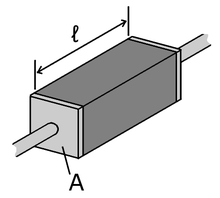
\includegraphics[scale=0.6]{../../questionBank/week05/q_resistivity_figs/wire.png}
    \end{center}
    \item Suppose we have $N$ such wires and align them side by side to form a mega-wire in the following fashion. Find the overall resistance of this mega-wire. What is this configuration similar to?
    \item Again, with $N$ identical wires, what's a configuration that can achieve the lowest resistance possible? What is this configuration similar to?
    \item Consider part (b) again, but this time, instead of $N$ copper wires, we split the number evenly between aluminum wires and copper wires, and we again align them side by side to form a mega-wire (with the left half all aluminum , and right half all copper). What's the overall resistance of this wire? (In terms of $\rho_{cu}, \rho_{Al}, L, $ and $a$)
    \item (Bonus) Instead of having all the $N/2$ copper wires on the right side, now all the wires are mixed together (a copper wire can be aligned right next to an aluminum wire), does the overall resistance of this new mega-wire change?
\end{enumerate}
